\documentclass[main.tex]{subfiles}

\begin{document}

\lstset{
  basicstyle=\ttfamily\small,
  backgroundcolor=\color{gray!10},
  frame=single,
  breaklines=true,
  breakindent=0pt,
  xleftmargin=2em,
  framexleftmargin=1em,
  literate=
    {é}{{\'e}}1 {è}{{\`e}}1 {ê}{{\^e}}1 {à}{{\`a}}1 {ç}{{\c{c}}}1
    {’}{{'}}1 {‘}{{'}}1
    {“}{{\textquotedbl}}1 {”}{{\textquotedbl}}1
    {"}{{\textquotedbl}}1
    {_}{{\_}}1
}


\section{Partie Antoine Canin}

\subsection{Introduction}

\quad Dans le cadre de notre projet de casiers sécurisés motorisés, plusieurs composants logiciels
et matériels ont dû être mis en œuvre pour assurer une communication fluide, sécurisée et
fonctionnelle entre les différentes parties du système. J’ai été en charge de plusieurs
aspects techniques essentiels à la réussite du projet : la mise en place d’une base de
données MariaDB accessible à distance, l’implémentation d’un lecteur RFID pour l’identification des utilisateurs, ainsi que la configuration d’un pare-feu IPFire afin de garantir
la sécurité du réseau. Cette section détaille les étapes réalisées, les choix techniques
effectués, ainsi que les justifications associées.

\subsection{Mise en place de la base de données}

\quad Afin de mener à bien le projet de Casier, la création d’une base de données était nécessaire, nous avons alors fait une base de données MariaDB.

Cette dernière a été installée sur une Raspberry Pi à l’aide des commandes suivantes :

\begin{lstlisting}
sudo apt-get update
// Commande permettant de mettre la Raspberry Pi à jour

sudo apt-get install mariadb-server
// Commande permettant d’installer l’agent MariaDB
\end{lstlisting}

Une fois installée, une configuration sécurisée a été effectuée avec :

\begin{lstlisting}
sudo mysql_secure_installation
// Commande permettant de sécuriser l’installation avec les options que l’on défini ci-dessous
\end{lstlisting}

Les options choisies lors de cette étape :

\begin{itemize}
\item Définir un mot de passe pour l’utilisateur root ;
\item Supprimer les utilisateurs anonymes ;
\item Désactiver l’accès root à distance ;
\item Supprimer la base de test ;
\item Recharger les privilèges.
\end{itemize}

Connexion à MariaDB :

\begin{lstlisting}
sudo mysql -u root -p
// Commande permettant de se connecter en administrateur sur MariaDB pour y ajouter des modifications
\end{lstlisting}

Création de la base et d’un utilisateur dédié :

\begin{lstlisting}
CREATE DATABASE m_Casier;
// Commande permettant de créer la base de données en l’appelant “m_Casier”

CREATE USER 'casier'@'localhost' IDENTIFIED BY 'casier';
// Commande permettant de créer l’utilisateur “casier”, il pourra se connecter uniquement depuis la machine locale avec le mot de passe “casier”

GRANT ALL PRIVILEGES ON m_Casier.* TO 'casier'@'localhost';
// Commande permettant de donner tous les privilèges à l’utilisateur “casier” sur la base de données “m_casier”

FLUSH PRIVILEGES;
// Commande permettant de recharger les privilèges avec ceux ci-dessus
\end{lstlisting}

Afin de permettre une interaction distante avec la base de données depuis le réseau, il a fallu modifier le fichier de configuration suivant :

\begin{lstlisting}
sudo nano /etc/mysql/mariadb.conf.d/50-server.cnf
\end{lstlisting}

Cette commande permet d’éditer le fichier de configuration se trouvant dans \textbf{/etc/mysql/mariadb.conf.d/} .

Changement de l’adresse d’écoute :

\begin{lstlisting}
bind-address = 0.0.0.0
// Commande permettant d’autoriser les connexions venant de toutes les adresses IP possible
\end{lstlisting}

Puis redémarrer le service :

\begin{lstlisting}
sudo systemctl restart mariadb
// Commande permettant de redémarrer MariaDB
\end{lstlisting}

Ajout des règles iptables pour n'autoriser que les connexions sur le port MySQL (3306) :

\begin{lstlisting}
sudo iptables -A INPUT -p tcp --dport 3306 -j ACCEPT
// Commande permettant d’autoriser toutes les connexions entrantes vers le port 3306 et concerne le port TCP

sudo iptables -A OUTPUT -p tcp --sport 3306 -j ACCEPT
// Commande permettant d’autoriser toutes les connexions sortantes dont le port source est 3306 (ce sont les réponses de MySQL), le serveur créé pourra donc répondre aux clients
\end{lstlisting}

Création de l’utilisateur pour les connexions distantes :

\begin{lstlisting}
CREATE USER 'casier'@'%' IDENTIFIED BY 'casier';
// Commande permettant de se connecter depuis n’importe quelle machine

GRANT ALL PRIVILEGES ON m_Casier.* TO 'casier'@'%' WITH GRANT OPTION;
// Commande permettant de donner tous les droits à             l’utilisateur

FLUSH PRIVILEGES;
// Commande permettant de se connecter à distance sur le serveur MySQL avec l’adresse IP 192.168.2.2

\end{lstlisting}

Pour accéder à la base depuis un poste client distant :

\begin{lstlisting}
mysql -h 192.168.2.2 -u casier -p
// Commande permettant d’afficher les bases de données existantes
\end{lstlisting}

Et pour vérifier que tout fonctionne :

\begin{lstlisting}
SHOW DATABASES;
// Commande permettant d’afficher les bases de données existantes

USE m_Casier;
// Commande permettant de rentrer dans la base de données
“m_Casier”

SHOW TABLES;
// Commande permettant de montrer les tables de la base de     données

SELECT * FROM Tag;
// Commande permettant de montrer tous les tags de la table
\end{lstlisting}

\textbf{Requête de vérification d’un badge dans la base :}

Lors de l’utilisation du système, il est nécessaire de vérifier si le badge scanné correspond à un badge déjà enregistré dans la base de données. Pour cela, une requête SQL de type SELECT COUNT(*) est utilisée via une requête préparée, afin d’éviter les injections SQL.

Le traitement a été implémenté côté application avec l’algorithme suivant (le code se trouvera en annexes) :

\begin{figure}[H]
	\centering
	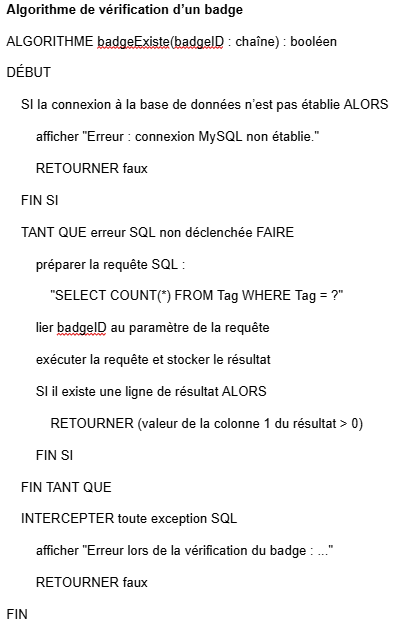
\includegraphics[width=0.6\textwidth]{../images/algoREQUETE}
	\caption{Algorithme de vérification d'un badge}
	\label{fig:AVB}
\end{figure}

\subsection{L'implémentation du lecteur RFID}

\quad Désormais, afin d’interagir avec la base de données, l’utilisation d’un lecteur RFID est cruciale, voici son implémentation dans le projet :

Nous allons vérifier la bonne communication entre le lecteur RFID (UEM4100) et la Raspberry Pi, et observer le format des données envoyées lors de la détection d’un badge.
\\ \\
Installation :

\begin{lstlisting}
sudo apt-get install picocom
// Commande permettant d’installer Picocom pour lire les badges
\end{lstlisting}

Pour identifier le port utilisé par le lecteur RFID (ex. /dev/ttyUSB0), on utilise :

\begin{lstlisting}
dmesg | grep tty
// Commande permettant d’afficher les messages du noyau, ceux contenant “tty”
\end{lstlisting}

Ce qui retourne des lignes comme :

\begin{lstlisting}
[    1.891679] fe201000.serial: ttyAMA1 at MMIO 0xfe201000 [...]
[    1.895232] fe215040.serial: ttyS0 at MMIO 0xfe215040 [...]
[    1.895304] printk: console [ttyUSB0] enabled
\end{lstlisting}

Dans notre cas, le port série était identifié comme /dev/ttyUSB0, mais un port peut apparaître comme /dev/ttyS0.

\textbf{Test du lecteur RFID avec Picocom :}

Avant d’intégrer le lecteur RFID série dans le programme principal, nous avons vérifié son bon fonctionnement à l’aide de Picocom, un utilitaire de communication série sous Linux. Après avoir connecté le lecteur RFID à la Raspberry Pi, la commande suivante permet permet de lire les données d’un badge, nous avons ensuite utilisé cette commande :

\begin{lstlisting}
picocom -b 9600 -d8 -p1 --imap 8bithex,nrmhex /dev/ttyUSB0
// Commande permettant de configurer la lecture avec une vitesse de 9600 bauds, 8 bits de données seront pris, la parité est mise à 1 et les caractères spéciaux pourront être affichés
\end{lstlisting}

Lorsque le badge est scanné, voici le format de trame observé :

\begin{lstlisting}
[02][32][36][30][30][42][34][33][45][46][46][35][33][03] (badge 1) 
[02][32][36][30][30][42][34][33][38][43][31][36][42][03] (badge 2)
\end{lstlisting}

Chaque badge est encadré par un octet [02] (STX) au début et [03] (ETX) à la fin. Seuls cinq octets hexadécimaux varient entre chaque badge, ce qui permet de les distinguer de manière fiable.

Commande pour lancer Picocom :

\begin{lstlisting}
picocom -b 9600 -fn -yn -d8 /dev/ttyUSB0
// Commande qui sera prise en priorité car plus courte et elle renvoie les mêmes données 
\end{lstlisting}

Explication des options :

-b 9600 : Débit en bauds (vitesse de transmission) \\
-fn : N'affiche pas les caractères non imprimables \\
-yn : Pas de contrôle de flux matériel \\
-d8 : Format série 8N1 (8 bits, No parity, 1 stop bit) \\
/dev/ttyUSB0 : Port série correspondant au lecteur

Exemple d’affichage obtenu lors du scan d’un badge :

\textbf{[02][32][36][30][30][42][34][33][45][46][46][35][33][03]}

Le badge est encadré par [02] (STX = début) et [03] (ETX = fin). Cinq octets hexadécimaux varient selon le badge, ce qui permet de les identifier de manière unique.

Ce test avec Picocom a permis de :

\begin{itemize}
\item Vérifier la bonne alimentation et connexion du lecteur RFID 
\item Observer le format brut des trames envoyées par les badges 
\item Déterminer les caractères utiles pour l’implémentation en C++
\end{itemize}

\textbf{Développement logiciel pour la lecture série}

Pour la lecture des badges via le port série, une classe C++ nommée RFIDReader a été développée. Cette classe, basée sur la bibliothèque serialib, permet de lire les trames transmises par le lecteur. Le badge est encadré par les caractères spéciaux STX (0x02) et ETX (0x03), ce qui facilite la détection du début et de la fin de la transmission. Le code est conçu pour extraire proprement les caractères utiles et retourner l’identifiant du badge sous forme de chaîne.

Algorithme de la méthode readBadge() (le code se trouvera en annexe) :

\begin{figure}[H]
	\centering
	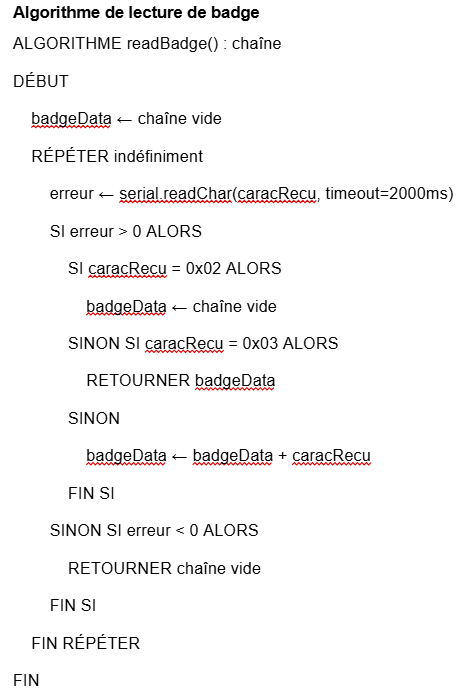
\includegraphics[width=0.6\textwidth]{../images/algoRFIDREADER}
	\caption{Algorithme de lecture de badge}
	\label{fig:ALB}
\end{figure}

\subsection{Complément sur la technologie RFID}

Dans le cadre du projet, une attention particulière a été portée au fonctionnement physique des systèmes RFID, afin de comprendre leur logique et d’optimiser leur intégration dans notre solution.

\textbf{Types de tags utilisés}

Le système utilise des tags passifs au format EM4100. Ces tags ne contiennent pas de batterie. Ils sont alimentés par le champ électromagnétique émis par le lecteur RFID, ce qui les rend particulièrement adaptés aux environnements industriels :

\begin{itemize}
\item Format : badge de type carte (épaisseur standard plastique)
\item Type : passif (sans source d’énergie autonome)
\item Mémoire : ROM contenant un identifiant unique non modifiable
\end{itemize}

Le lecteur utilisé dans notre projet fonctionne à la fréquence de 125 kHz, qui fait partie des basses fréquences (LF) dans la classification RFID.

Les caractéristiques de cette bande sont :

\begin{itemize}
\item Portée de lecture courte (2 à 10 cm)
\item Très bonne résistance aux interférences métalliques ou liquides
\item Débit de données modéré mais suffisant pour de l’identification simple
\end{itemize}

Ce choix est particulièrement adapté à une application sécurisée et contrôlée, comme l’ouverture de casiers d’accès physique.

\textbf{Comment fonctionne le badge RFID ?}

Sur le plan physique, le badge RFID fonctionne selon le principe de l’induction électromagnétique :

\begin{itemize}
\item Le lecteur génère un champ magnétique oscillant à 125 kHz
\item Lorsqu’un badge entre dans ce champ, sa bobine interne capte l’énergie, alimente brièvement la puce RFID, et celle-ci émet une réponse
\item Cette réponse contient l’identifiant unique du tag, transmis par modulation de charge (type ASK ou FSK selon les modèles)
\end{itemize}

Cette transmission est unidirectionnelle (tag → lecteur), rapide (environ quelques millisecondes) et ne nécessite aucun contact physique.

\textbf{Avantages et inconvénients de la RFID 125 kHz}

\begin{table}[h!]
\centering
\begin{tabular}{|p{7cm}|p{7cm}|}
\hline
\textbf{Avantages} & \textbf{Inconvénients} \\
\hline
Lecture sans contact, même à travers des surfaces & Portée de lecture courte (jusqu’à 10 cm) \\
\hline
Pas de pile dans les badges & Usage limité à l’identification \\
\hline
Robuste face aux chocs & Impossible de modifier la donnée du badge \\
\hline
Très faible coût & Nécessite une proximité et un bon alignement du badge \\
\hline
\end{tabular}
\end{table}

Cette technologie, bien que simple, répond parfaitement aux besoins de notre système : identification rapide, fiable et sécurisée, sans contrainte de maintenance ni risque de panne liée à une alimentation embarquée dans les tags.

Enfin, j’ai approfondi les principes physiques à l’origine de la technologie RFID, notamment l’induction électromagnétique et la modulation de charge. Le choix des tags passifs à 125 kHz s’est révélé pertinent pour une lecture fiable à courte distance, bien adaptée au contexte industriel. Malgré une portée limitée, ce système offre une solution économique, sans entretien et facile à intégrer dans une chaîne automatisée

\subsection{Configuration du Pare-Feu}

\quad Pour assurer la sécurité et le cloisonnement de notre réseau, nous avons installé un pare-feu IPFire sur un NUC. L’installation a débuté par la création d’une clé USB bootable à l’aide du logiciel balena Etcher, que nous avons lancé en mode administrateur. Après avoir sélectionné l’image ISO d’IPFire, nous avons généré la clé puis démarré le NUC en accédant au BIOS via la touche F11.

L’installation a été lancée en mode UEFI, et nous avons procédé aux réglages initiaux, notamment le choix de la langue, du clavier, ainsi que la définition du nom de domaine ipfire.sylvamo. Le compte administrateur root a été défini avec le mot de passe passwd, ce mot de passe a été utilisé pour une phase de test mais doit être nettement plus complexe pour une utilisation réelle.

Nous avons opté pour une configuration en trois zones : GREEN, RED et ORANGE. Pour affecter correctement les interfaces réseau à ces zones, nous avons utilisé la commande dmesg immédiatement après le branchement d’un câble Ethernet, ce qui nous a permis d’identifier les ports grâce aux messages système, une opération nécessitant rapidité et précision. Les adresses MAC des interfaces ont été notées afin d’éviter toute confusion lors de l’attribution des zones. La zone RED correspond au réseau d’entreprise, la zone GREEN correspond au réseau dans lequel seront les machines du projet, pour finir, la zone ORANGE contiendra la base de données, c’est donc la zone démilitarisée.

Une fois l’installation terminée, nous avons accédé à l’interface web d’IPFire depuis un poste situé en zone verte, à l’adresse https://192.168.1.1:444, avec les identifiants admin et passwd. Plusieurs configurations ont ensuite été réalisées : nous avons spécifié l’adresse DNS 10.187.52.5 dans la section réseau, puis indiqué un serveur NTP dans les paramètres de synchronisation horaire. L’accès SSH a été activé et paramétré pour autoriser l’authentification par mot de passe.

Sur le poste client, nous avons généré une paire de clés SSH de type ed25519, sans mot de passe, grâce à la commande ssh-keygen. La clé publique a été transférée sur la machine IPFire à l’aide de ssh-copy-id. Afin de garantir un accès sécurisé, nous avons créé le répertoire .ssh sur le NUC, ajusté les permissions nécessaires, puis inscrit la clé dans le fichier authorized\_keys.

Le serveur DHCP a ensuite été configuré pour la zone verte, avec une plage d’adresses allant de 192.168.1.100 à 192.168.1.110. Enfin, nous avons attribué une adresse IP statique à la Raspberry Pi connectée à la zone orange via l’outil nmtui, en utilisant les paramètres suivants : 192.168.2.2/24 pour l’adresse IP, 192.168.2.1 pour la passerelle, et 9.9.9.9 comme serveur DNS.

La mise en place du pare-feu s’est terminée par la création de deux règles spécifiques : la première autorise le trafic TCP depuis la zone verte vers la zone orange sur le port 3306 (port MySQL), tandis que la seconde autorise l’ensemble des protocoles depuis la zone rouge vers la zone orange. Ces deux règles ont été appliquées et enregistrées via l’interface de gestion d’IPFire.

Voici à quoi ressemble le réseau :

\begin{figure}[H]
	\centering
	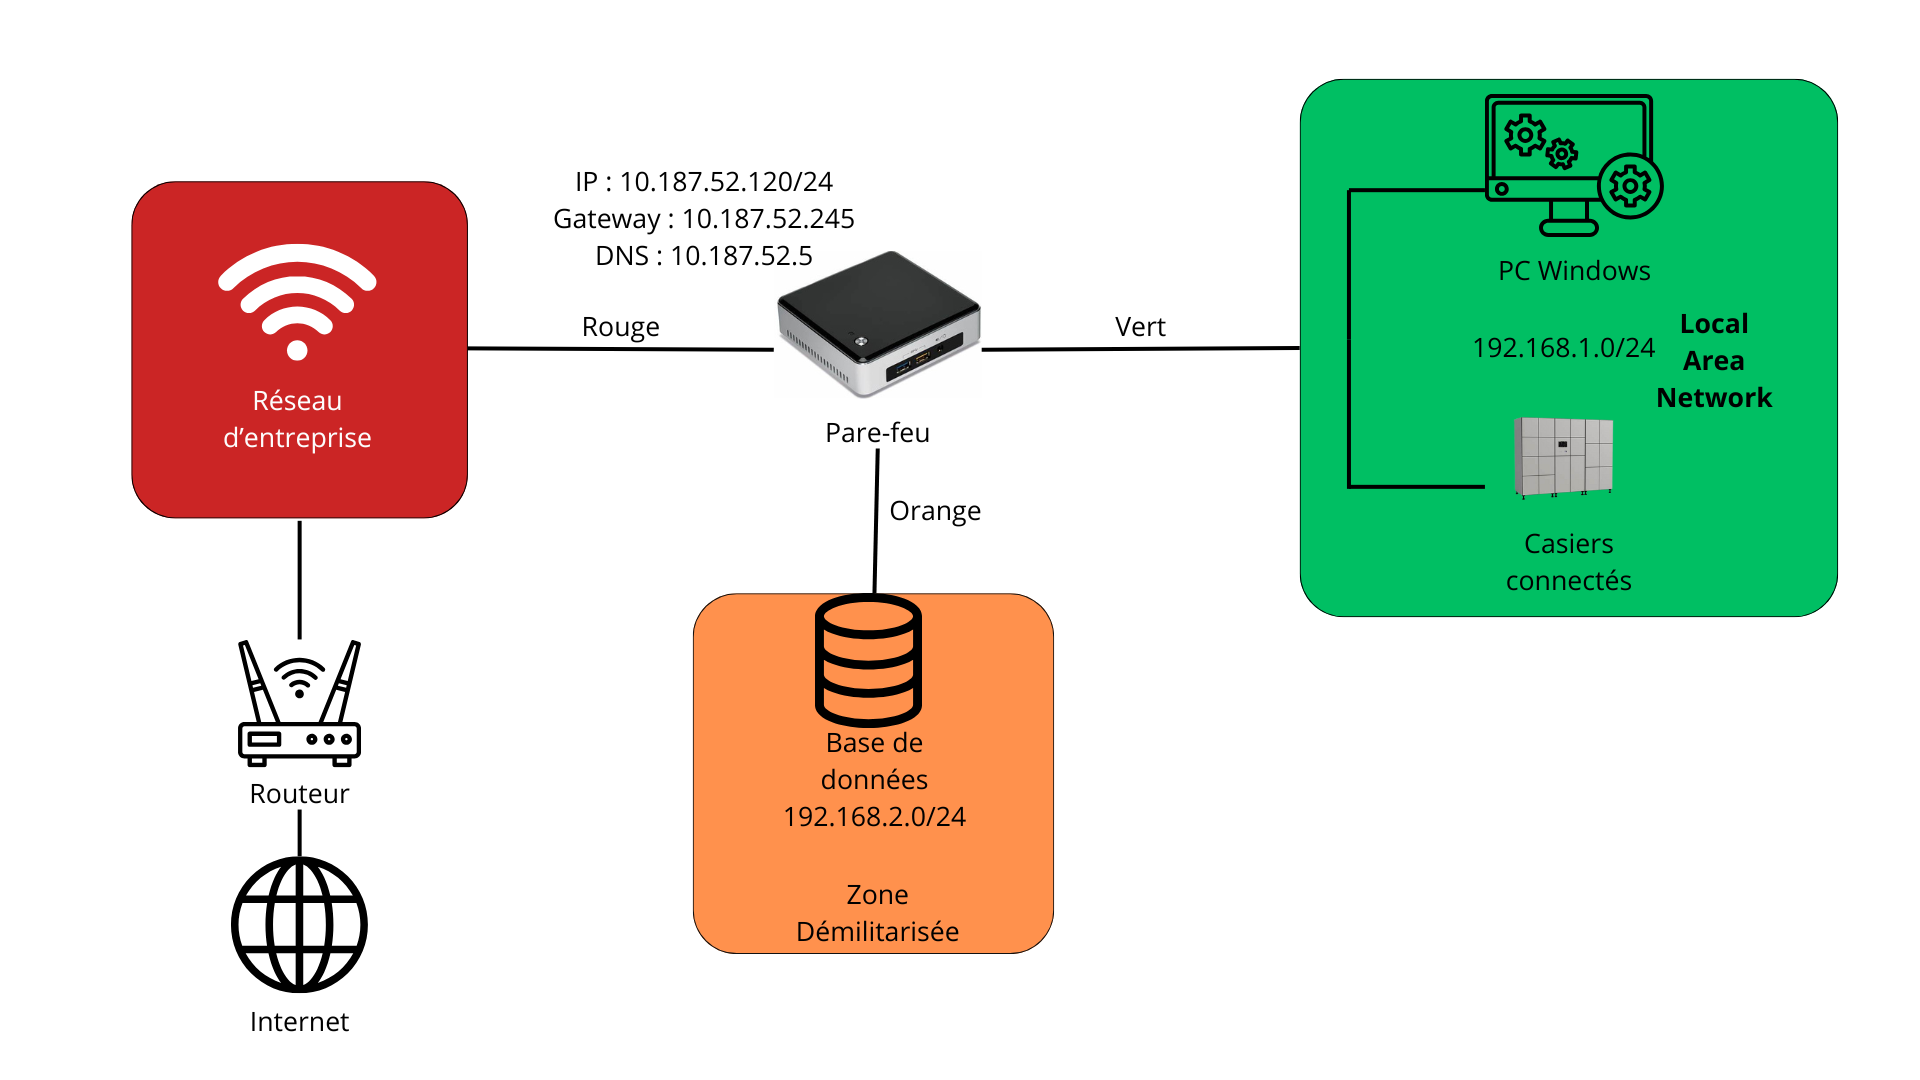
\includegraphics[width=0.6\textwidth]{../images/AccèsInternet}
	\caption{Vue d'ensemble du réseau}
	\label{fig:VER}
\end{figure}

\newpage

\end{document}